% \documentclass[bwprint]{cumcmthesis} %去掉封面与编号页
% \documentclass{cumcmthesis}
\documentclass[withoutpreface,bwprint]{cumcmthesis} %去掉封面与编号页
\newcommand{\diff}{\mathop{}\!\mathrm{d}} % 正体微分符号

\usepackage{graphicx}       % 用于插入图片
\usepackage{subcaption} 
\usepackage{algorithm}
\usepackage{algorithmic} % 导言区需添加这两个宏包
\usepackage{comment}  

\usepackage{booktabs}
\usepackage{tabularx}
\usepackage{float}
\usepackage{threeparttable} % 表,图注
\usepackage[numbers]{natbib}
\usepackage[table]{xcolor}      % 颜色选项

\title{基于 的 模型}
\tihao{A}
\baominghao{}
\schoolname{中原工学院}
\membera{}
\memberb{}
\memberc{}
\supervisor{魏冰蔗}
\yearinput{2025}
\monthinput{09}
\dayinput{07}


\begin{document}

% 标题
\maketitle
\nocite{*}
\bibliographystyle{gbt7714-numerical}

% 第三条 论文第三页为摘要专用页。摘要内容(含标题和关键词,无需翻译成英文)不能超过一页;论文从此页开始编写页码,页码位于页脚中部,用阿拉伯数字从“1”开始连续编号。
\begin{abstract}
本文

    \textbf{针对问题一,}

    \textbf{针对问题二,}

    \textbf{针对问题三,}

    \textbf{针对问题四,}

    \keywords{红外干涉法\quad 多光束干涉\quad Snell定律\quad 菲涅耳公式}
\end{abstract}

% 论文从第四页开始是正文内容(不要目录,尽量控制在20页以内);正文之后是论文附录(页数不限),附录内容必须打印并与正文装订在一起提交。
% 问题背景与重述
\section{问题重述}

\subsection{问题背景}
碳化硅作为第三代半导体材料的代表,因其优异的综合性能备受关注。碳化硅外延层厚度是外延材料的关键参数,直接影响器件性能。因此,建立科学、准确、可靠的厚度测试标准至关重要。红外干涉法是一种无损测量方法,其原理基于外延层与衬底因掺杂载流子浓度不同而具有不同的折射率。红外光入射外延层后,部分光从外延层表面反射,部分光从衬底表面反射回来,两束光在特定条件下产生干涉条纹。通过红外光谱的波长、外延层折射率及入射角等参数,可确定外延层厚度。需要注意的是,外延层折射率通常不是常数,与掺杂载流子浓度及红外光波长等因素相关。

\subsection{问题提出}

\textbf{问题1:}在考虑外延层和衬底界面只有一次反射、透射所产生的干涉条纹的情况下,建立确定外延层厚度的数学模型。

\textbf{问题2:}根据问题一建立的确定外延层厚度数学模型,设计其对应的算法,根据提供的碳化硅晶圆片的光谱实测数据求出计算结果,并分析计算结果的可靠性。

\textbf{问题3:}光波在外延层和衬底界面可能发生多次反射和透射,形成多光束干涉。推导多光束干涉的必要条件及其对外延层厚度计算精度的潜在影响。基于多光束干涉的条件,分析提供的硅晶圆片测试结果是否出现多光束干涉,建立硅外延层厚度计算的数学模型和算法,并给出计算结果。若碳化硅晶圆片测试结果中也存在多光束干涉,影响厚度计算精度,提出消除多光束干涉影响的方法,并给出消除影响后的计算结果。


% 问题分析
\section{问题分析}

\subsection{问题一分析}

\subsection{问题二分析}
\begin{algorithm}
\caption{碳化硅外延层厚度计算算法}
\begin{algorithmic}[1]
\REQUIRE 附件文件路径, $n$, $\theta$
\ENSURE 外延层厚度厚度$d(\mu m)$, 可靠性指标
\STATE $\sigma$, $R$ $\gets $\text{ReadXLSX}(文件路径)   \% 读取波数和反射率
\STATE $R$ $\gets$ \text{BaselineCorrect}($R$)  \% 基线校正 (e.g., 扣 min(R), 归一如果 >100\%)
\STATE $R_{smooth}$ $\gets$ \text{SavgolFilter}($R$, window=21, order=2)  \% 平滑去噪
\STATE $valley_{indices}$ $\gets$ \text{FindPeaks}($-R_{smooth}$, distance=250, prominence=5)  \% 检测谷位置
\IF {$length(valley_{indices}) < 2$}
    \STATE $d$ $\gets$ \text{NaN}  \% 条纹不足, 切换FFT方法
    \STATE $f$ $\gets$ \text{FFTMainFreq}(R - mean(R))  \% FFT提取主频
    \STATE $d$ $\gets$ $10^4 / (2 f \sqrt{n^2 - \sin^2 \theta})$
\ELSE
    \STATE $valley_{\sigma} \gets \sigma[valley_{indices}]$
    \STATE $\Delta\sigma \gets \text{Diff}(valley_{\sigma})$  \% 相邻差
    \STATE $avg_{\Delta\sigma} \gets \text{Mean}(\Delta\sigma) $ \% 平均 (忽略异常)
    \STATE $cos_{term} \gets \sqrt{n^2 - \sin^2 \theta}$
    \STATE $d \gets 10^4 / (2 \cdot avg_{\Delta\sigma} \cdot cos_{term})  \% \mu m$
\ENDIF
\STATE $rel_{error}$ $\gets$ $|d_1 - d_2| / ((d_1 + d_2)/2)$  \% 多角度一致性
\STATE $\text{AnalyzeSensitivity}(d, \delta n=0.01, \delta \theta=0.5^\circ$)  \% 敏感性
\RETURN $d$, $rel_{error}$
\end{algorithmic}
\end{algorithm}

\subsection{问题三分析}

% 模型假设
\section{模型假设}

\begin{enumerate}
    \item 假设光源为偏振光,振幅可调节
    \item 
    \item 
\end{enumerate}

% 符号说明
\section{符号说明}

% 表结构
\begin{table}[H]
    \centering  % 表居中
    \caption{符号说明详表}  % 表标题
    \label{tab:符号说明}  % 表标签
    \begin{threeparttable}
        % 表内容
        \begin{tabularx}{\textwidth}{p{0.15\textwidth} p{0.7\textwidth} l}
            \toprule[1.5pt]
            \textbf{符号} & \textbf{说明} & \textbf{单位} \\ 
            \midrule[1pt]
            $A, B, C$ & 柯西等式未知量符号表达式 & - \\
            $\theta_1$ & 入射角的角度 & rad \\
            $\theta_2$ & 折射角的角度 & rad \\
            $\theta_3$ & 反射角的角度 & rad \\
            $c$ & 光速,取299,792,458m/s & m/s \\
            $\tilde{v} $ & 波数 & m$^{-1}$\\
            $\nu$ & 光的频率 & Hz\\
            $\lambda$ & 光的波长 & m\\
            $n_0$ & 空气的折射率 & - \\
            $n_1$ & 外延层的折射率 & - \\
            $n_2$ & 碳化硅(SiC)的折射率 & - \\
            $\delta$ & 相位差 & m \\
            $R$ & 反射率 & \% \\  

            \bottomrule[1.5pt]
        
        \end{tabularx}
        \begin{tablenotes}
            \footnotesize
            \item 注:其他文章内使用但未在表内详细说明的符号将在使用时给出说明。
        \end{tablenotes}
    \end{threeparttable}
\end{table}




% 模型建立与求解
\section{模型建立与求解}
\subsection{问题一}
\subsubsection{模型建立}
\begin{figure}[H]
    \centering
    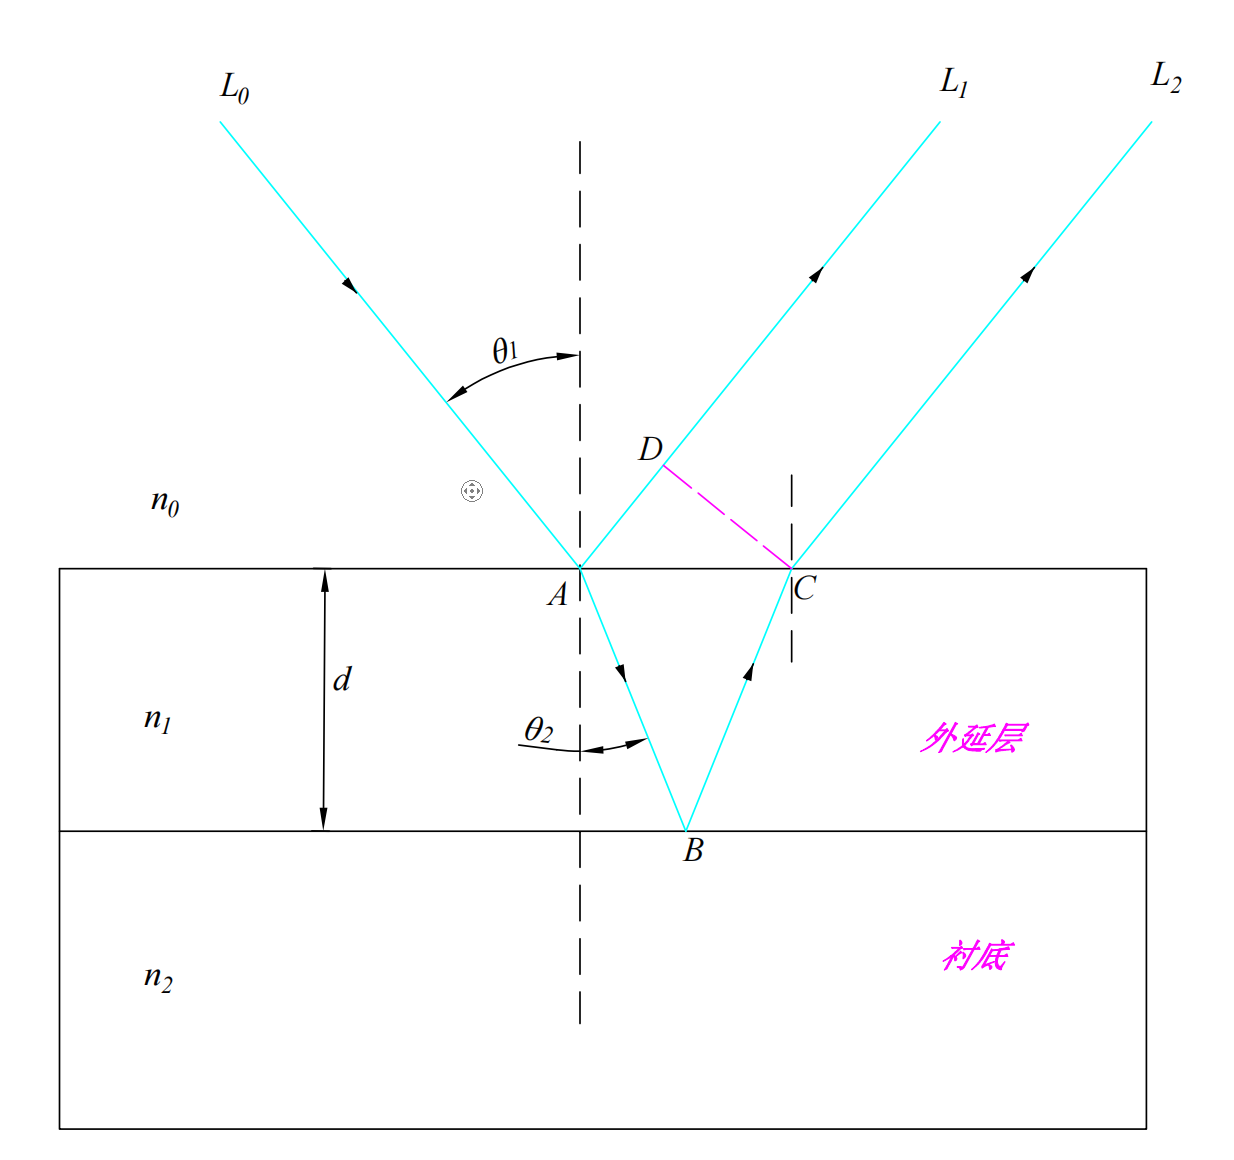
\includegraphics[width=0.6\textwidth]{../figure/q1.png}
    \caption{外延层红外反射示意图}
    \label{fig:外延层红外反射示意图}
\end{figure}
图\ref{fig:外延层红外反射示意图}为外延层红外反射示意图。

由于外延层上下表面反射的两束相干光$L_1$和$L_2$存在相位差,其光程差导致了干涉条纹的形成。


1、几何光程


2、光程差分析
\begin{equation}
    \Delta X = n_1(AB + BC) - n_0AD = 2 n_1 d \cos \theta_2
\end{equation}

2、相位差
Δϕ=2πλ⋅ΔX+Δϕreflect


。


$n_1 > n_2$,图\ref{fig:外延层红外反射示意图}中,$L_1$在A点会发生$\pi$的反射相变,$L_2$在B点的反射相变为$0$,$L_2$在C点的折射线和反射线的相位均与BC入射线相同,则有干涉条件方程组
\begin{equation}
    \begin{cases}
        \text{相长干涉} & \Delta X = m\lambda_m,  m=0,1,2,… \\
        \text{相消干涉} & \Delta X = (m+\frac{1}{2}) \lambda_m,  m=0,1,2,… 
    \end{cases}
\end{equation}


\subsubsection{问题求解}
\subsubsection{求解结果}

\subsection{问题二}
\subsubsection{模型建立}
\subsubsection{问题求解}
\subsubsection{求解结果}

\subsection{问题三}
\subsubsection{模型建立}
\subsubsection{问题求解}
\subsubsection{求解结果}

% 模型的分析与检验
\section{模型的分析与检验}
\subsection{误差分析}
\subsection{灵敏度分析}


% 模型评价
\section{模型的评价}
\subsection{模型优点}
\begin{enumerate}
    \item 
    \item 
    \item 
\end{enumerate}

\subsection{模型缺点}
\begin{enumerate}
    \item 
    \item 
\end{enumerate}

\subsection{改进方向}
\begin{enumerate}
    \item 
    \item 
\end{enumerate}

% 所有引用他人或公开资料(包括网上资料)的成果必须按照科技论文的规范列出参考文献,并在正文引用处予以标注。
\bibliography{ref}

\newpage
% 附录
% 论文附录内容应包括支撑材料的文件列表,建模所用到的全部完整、可运行的源程序代码(含EXCEL、SPSS等软件的交互命令)等。如果缺少必要的源程序、程序不能运行或运行结果与论文不符,都可能会被取消评奖资格。如果确实没有用到程序,应在论文附录中明确说明“本论文没有用到程序”。
\begin{appendices}

\section{运行结果}
\subsection{点集合}
\begin{table}[H]
    \centering  % 表居中
    \caption{数据1}  % 表标题
    \label{tab:数据1}  % 表标签
    \begin{threeparttable}
        % 表内容
        \begin{tabularx}{\textwidth}{c |c c | c c | c c}
            \toprule[1.5pt]
            $\theta_1$& \textbf{波数(cm$^{-1}$)} & \textbf{反射率(\%)} & \textbf{波数(cm$^{-1}$)}  & \textbf{反射率(\%)} & \textbf{波数(cm$^{-1}$)} & \textbf{反射率(\%)}   \\ 
            \midrule[1pt]
            \multirow{5}{*}{$10^\circ$}& 400.1569 &    31.2932 &   517.7933 &    33.8907 &    636.394 &     35.881\\
            & 832.6155 &     95.385 &   1012.445 &    4.67879 &   1085.727 &    9.43943\\
            & 1216.38 &    13.3879 &   1401.513 &    15.4973 &   1595.324 &    16.6738\\
            & 1836.865 &    17.5385 &   2079.851 &    17.9926 &   2322.356 &    18.1737\\
            & 2586.074 &    18.3814 & \\
            \midrule[1pt]
            \multirow{5}{*}{$15^\circ$} & 400.1569 &    36.3367 &   519.7218 &    36.8981 &   639.7689 &    39.0793\\
            & 927.5925 &    99.9829 &   988.3392 &    8.82083 &   1088.137 &    10.7283\\
            & 1221.684 &    14.3203 &   1416.459 &    16.4243 &   1607.377 &    17.4551\\
            & 1866.756 &    18.3449 &   2089.976 &    18.7524 &    2389.37 &    18.6991\\
            & 2617.411 &    19.1469 & \\

            \bottomrule[1.5pt]
        
        \end{tabularx}
    \end{threeparttable}
\end{table}



\section{文件列表}
\begin{table}[H]
    \caption{程序文件列表}
    \centering
    \begin{tabularx}{\textwidth}{c l}
        \bottomrule[1.5pt]
        文件名 & 功能描述 \\
        \midrule[1pt]
        code2.py & 问题二程序代码 \\
        code3.py & 问题三程序代码 \\
        \bottomrule[1.5pt]
    \end{tabularx}
    \label{tab:文件列表}
\end{table}

\section{代码}

\subsection{问题2代码}
\lstinputlisting[language=python]{../code/code2.py}

\subsection{问题3代码}
\lstinputlisting[language=python]{../code/code3.py}

\end{appendices}

\end{document}